\documentclass{beamer}
\usepackage{polski}
\usepackage[utf8]{inputenc}
\usetheme{Madrid}
\date{}
\title{}
\begin{document}
\begin{frame}{.}
	\begin{center}
	
\includegraphics[width=0.5\linewidth]{kernel.jpg}\\
	Opiekunem koła jest:\\
	Dr inż. Antoni Dydejczyk\\
	
\includegraphics[width=0.1\linewidth]{agh.jpg}
	\hspace{20em}
	
\includegraphics[width=0.1\linewidth]{fis.jpg}
	\end{center}
\end{frame}
\begin{frame}{O nas}
	\begin{minipage}[0.2\textheight]{\textwidth}
	\begin{columns}[T]
	\begin{column}{0.6\textwidth}
	\begin{itemize}
	\item Działamy na Wydziale Fizyki i Informatyki Stosowanej już od 10 lat
	\item Ponad 20 zarejestrowanych członków
	\item Zrealizowane liczne ciekawe projekty oraz wiele w przygotowaniu
	\item Wiele możliwości rozwoju i poszerzania wiedzy
	\item Dobra zabawa we wspaniałym gronie
	\end{itemize}
	\end{column}
	\begin{column}{0.2\textwidth}
	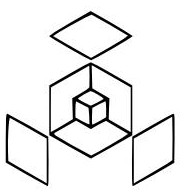
\includegraphics[width=3cm]{kernel_mini.jpg}
	\end{column}
	\end{columns}
	\end{minipage}
\end{frame}
\begin{frame}{Obecna działalność}
	\begin{minipage}[0.2\textheight]{\textwidth}
	\begin{columns}[T]
	\begin{column}{0.6\textwidth}
	\begin{itemize}
	\item Organizacja wykładów o tematyce informatycznej
	\item MISIO - Modularny Interaktywny System Informatycjo Organizacyjny
	\item Warsztaty "Ośla łączka Pythona", "Akademia Linuxa" oraz "Sieci komputerowe"
	\item Współpraca z kołem "Bozon" przy budowie i oprogramowywaniu radioteleskopu
	\item Szeroko rozwinięta współpraca z Krakowską Grupą Użytkowników Linuksa (CLUG)
	\end{itemize}
	\end{column}
	\begin{column}{0.5\textwidth}
	\vspace{0.5cm}
	\hspace{-0.8cm}
	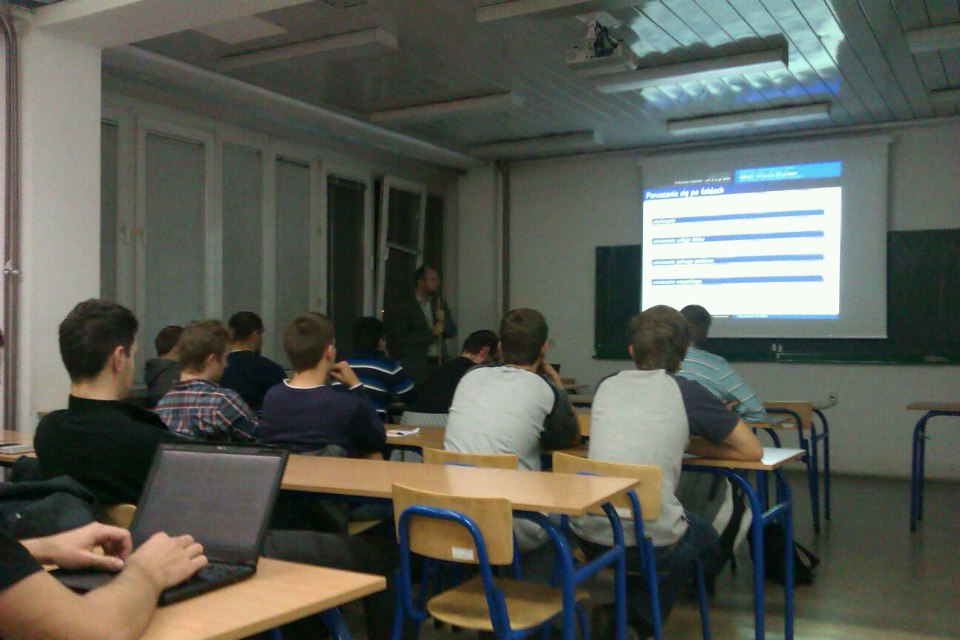
\includegraphics[width=6cm]{wyklad.jpg}\\
	\vspace{0.5cm}
	\hspace{-0.8cm}
	
\includegraphics[width=6cm]{clug.png}
	\end{column}
	\end{columns}

	\end{minipage}
\end{frame}
\begin{frame}{Czym dysponujemy}
	\begin{minipage}[0.2\textheight]{\textwidth}
	\begin{columns}[T]
	\begin{column}{0.5\textwidth}
	\begin{itemize}
	\item Reksio - serwer stworzony specjalnie na potrzeby koła i przeznaczony głównie do wspierania procesu tworzenia oprogramowania
	\item Konsola Play Station 3 - wysokowydajna maszyna obliczeniowa, procesor Cell Wyposażony w 8 rdzeni z zainstalowanym systemem Linux
	\item Ciągle rozszerzające się zbiory książek biblioteki Koła
	\end{itemize}
	\end{column}
	\begin{column}{0.5\textwidth}
	\vspace{0.5cm}
	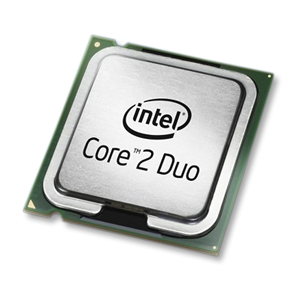
\includegraphics[width=6cm]{procesor.jpg}\\
	\end{column}
	\end{columns}

	\end{minipage}
\end{frame}
\begin{frame}{Plany na przyszłość}
	\begin{minipage}[0.2\textheight]{\textwidth}
	\begin{columns}[T]
	\begin{column}{0.5\textwidth}
	\begin{itemize}
	\item Kontynuacja cyklu wykładów LUMD
	\item Rozwój aktualnych projektów
	\item Poszerzanie wiedzy podczas warsztatów i konferencji
	\item Współpraca z Hackerspace-krk oraz wykonywanie wspólnych projektów
	\item Organizacja studenckich konferencji informatycznych
	\end{itemize}
	\end{column}
	\begin{column}{0.5\textwidth}
	\vspace{0.5cm}
	
\includegraphics[width=6cm]{TUX.png}\\
	\end{column}
	\end{columns}

	\end{minipage}
\end{frame}
\end{document}
